\documentclass[12pt,a4paper]{article}
\usepackage[utf8]{inputenc}
\usepackage[margin=1in]{geometry}
\usepackage{graphicx}
\usepackage{float}
\usepackage{amsmath}
\usepackage{listings}
\usepackage{xcolor}
\usepackage{enumitem}

% Code listing style
\lstset{
		language=C++,
		basicstyle=\ttfamily\footnotesize,
		keywordstyle=\color{blue},
		commentstyle=\color{green},
		stringstyle=\color{red},
		numbers=left,
		numberstyle=\tiny,
		frame=single,
		breaklines=true
}

\begin{document}

% Front Page
\begin{titlepage}
	\centering
	\vspace*{3cm}

	{\Huge\bfseries CSE 406 \textendash{} Lab Report: Least Recently Used (LRU) Page Replacement \par}
	\vspace{2.5cm}

	\noindent
	\begin{minipage}[t]{0.48\textwidth}
		{\large\bfseries Submitted By:}\\[0.5em]
		\Large
		Sharif Md. Yousuf \\
		ID: 22101128 \\
		Section: C-2 \\
		4th Year, 1st Semester \\
		Spring 2025
	\end{minipage}
	\hfill
	\begin{minipage}[t]{0.48\textwidth}
		{\large\bfseries Submitted To:}\\[0.5em]
		\Large
		Atia Rahman Orthi \\
		Lecturer \\
		Department of Computer Science \& Engineering \\
		University of Asia Pacific
	\end{minipage}

	\vfill

	{\Large\bfseries Date of Submission:} \\[0.5em]
	{\LARGE\bfseries 9 October, 2025 (Thursday)}

	\vspace*{2cm}
\end{titlepage}

\section{Problem Statement}
In this lab, I implemented a demand paging simulator that applies the Least Recently Used (LRU) page replacement strategy. The program receives an initial configuration and then processes a complete reference string, replacing pages based on how recently they were accessed. The tool must trace each reference, track the content of the frames, and compute overall hit/fault statistics.

\subsection*{Input}
For this experiment, I worked with the following configuration:
\begin{itemize}
	\item Frame size: 4 frames
	\item Number of page references: 11
	\item Page reference string
\end{itemize}

\begin{verbatim}
7 0 1 2 0 3 0 4 2 3 0
\end{verbatim}

\subsection*{Output}
My simulator prints the frame state after every access and aggregates the final performance statistics. A sample run with the above parameters produces:
\begin{verbatim}
Page Reference | Frames Status | Hit/Miss
--------------------------------------------
			7        | [7] [ ] [ ] [ ] | MISS
			0        | [7] [0] [ ] [ ] | MISS
			1        | [7] [0] [1] [ ] | MISS
			2        | [7] [0] [1] [2] | MISS
			0        | [7] [0] [1] [2] | HIT
			3        | [3] [0] [1] [2] | MISS
			0        | [3] [0] [1] [2] | HIT
			4        | [3] [0] [4] [2] | MISS
			2        | [3] [0] [4] [2] | HIT
			3        | [3] [0] [4] [2] | HIT
			0        | [3] [0] [4] [2] | HIT

====== RESULTS ======
Total Page Requests: 11
Total Page Hits: 5
Total Page Faults: 6
Hit Ratio: 45.45%
Fault Ratio: 54.55%
\end{verbatim}

\section{Objective}
Through this lab, I aimed to:
\begin{itemize}
		\item Understand the mechanics behind the LRU page replacement policy
		\item Implement an accurate frame tracking system that updates recency information on every access
		\item Measure hit/fault statistics for a fixed reference string and memory size
		\item Contrast LRU behaviour with FIFO and MRU policies explored in earlier labs
		\item Appreciate how LRU improves hit ratio by evicting the page that has been unused the longest
\end{itemize}

\section{Source Code Screenshot}
\begin{figure}[H]
	\centering
	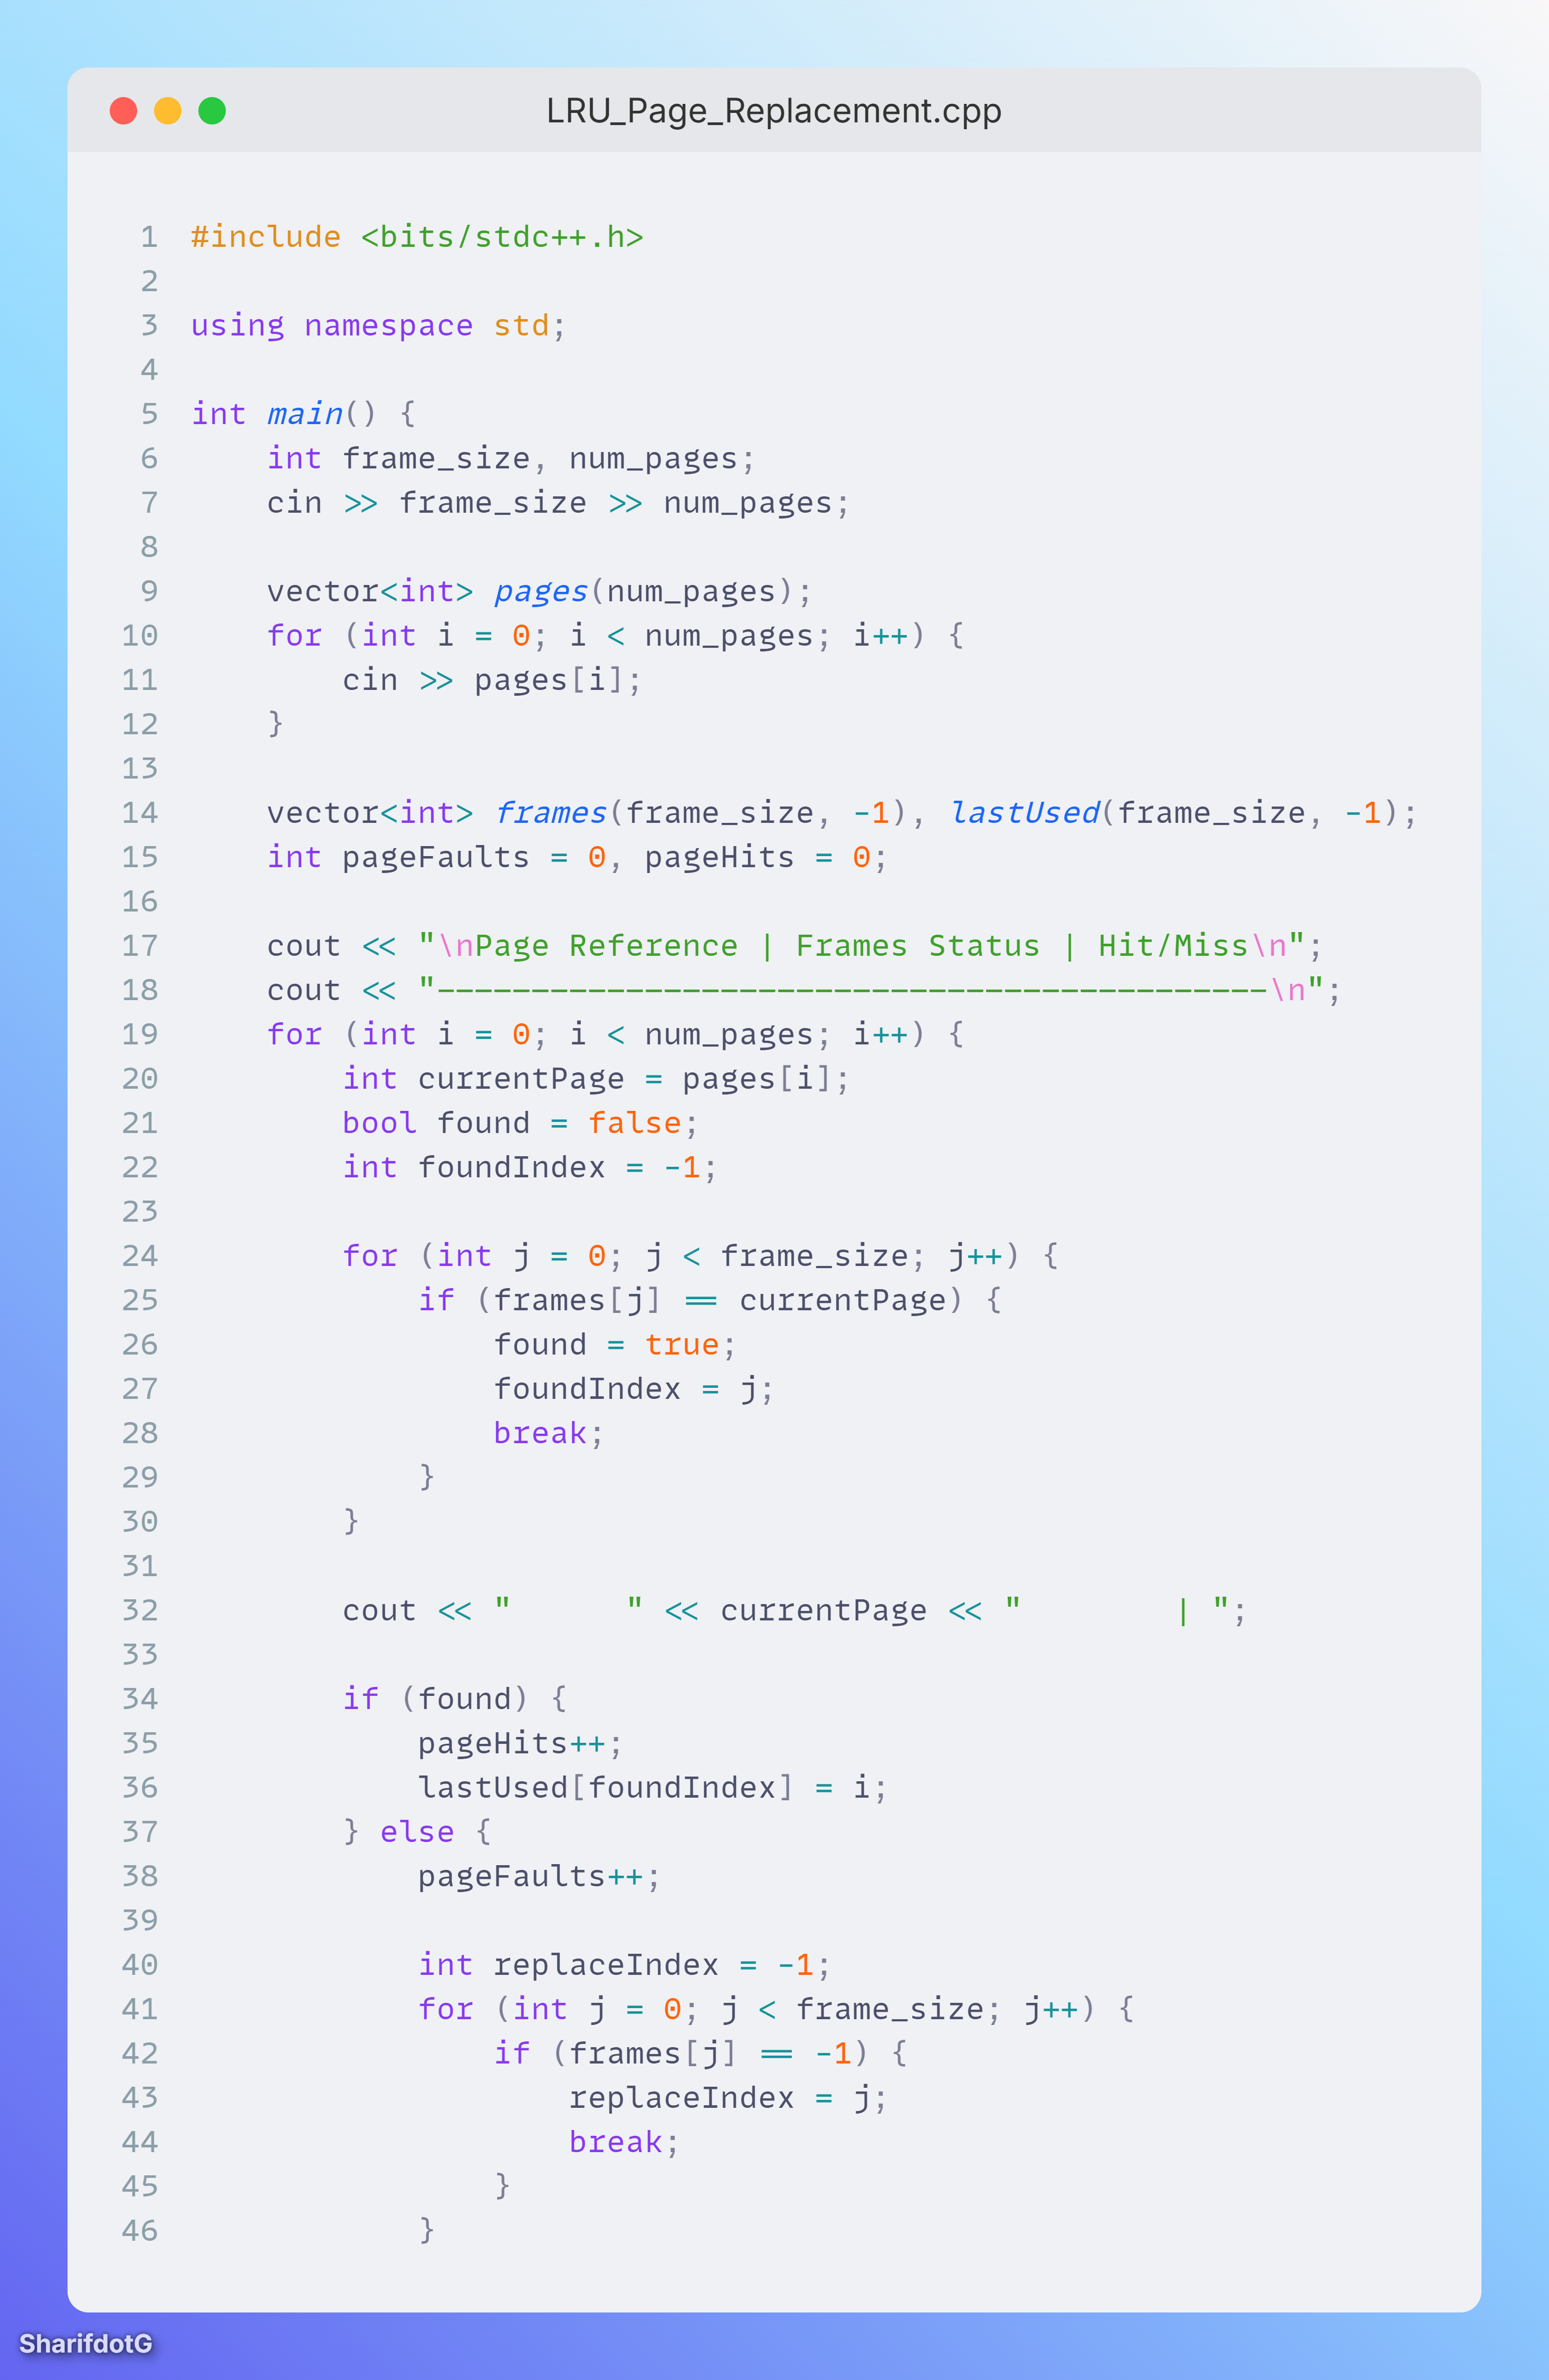
\includegraphics[width=0.85\textwidth]{Code1.png}
	\caption{LRU Page Replacement Source Code (Part 1)}
\end{figure}

\begin{figure}
    \centering
    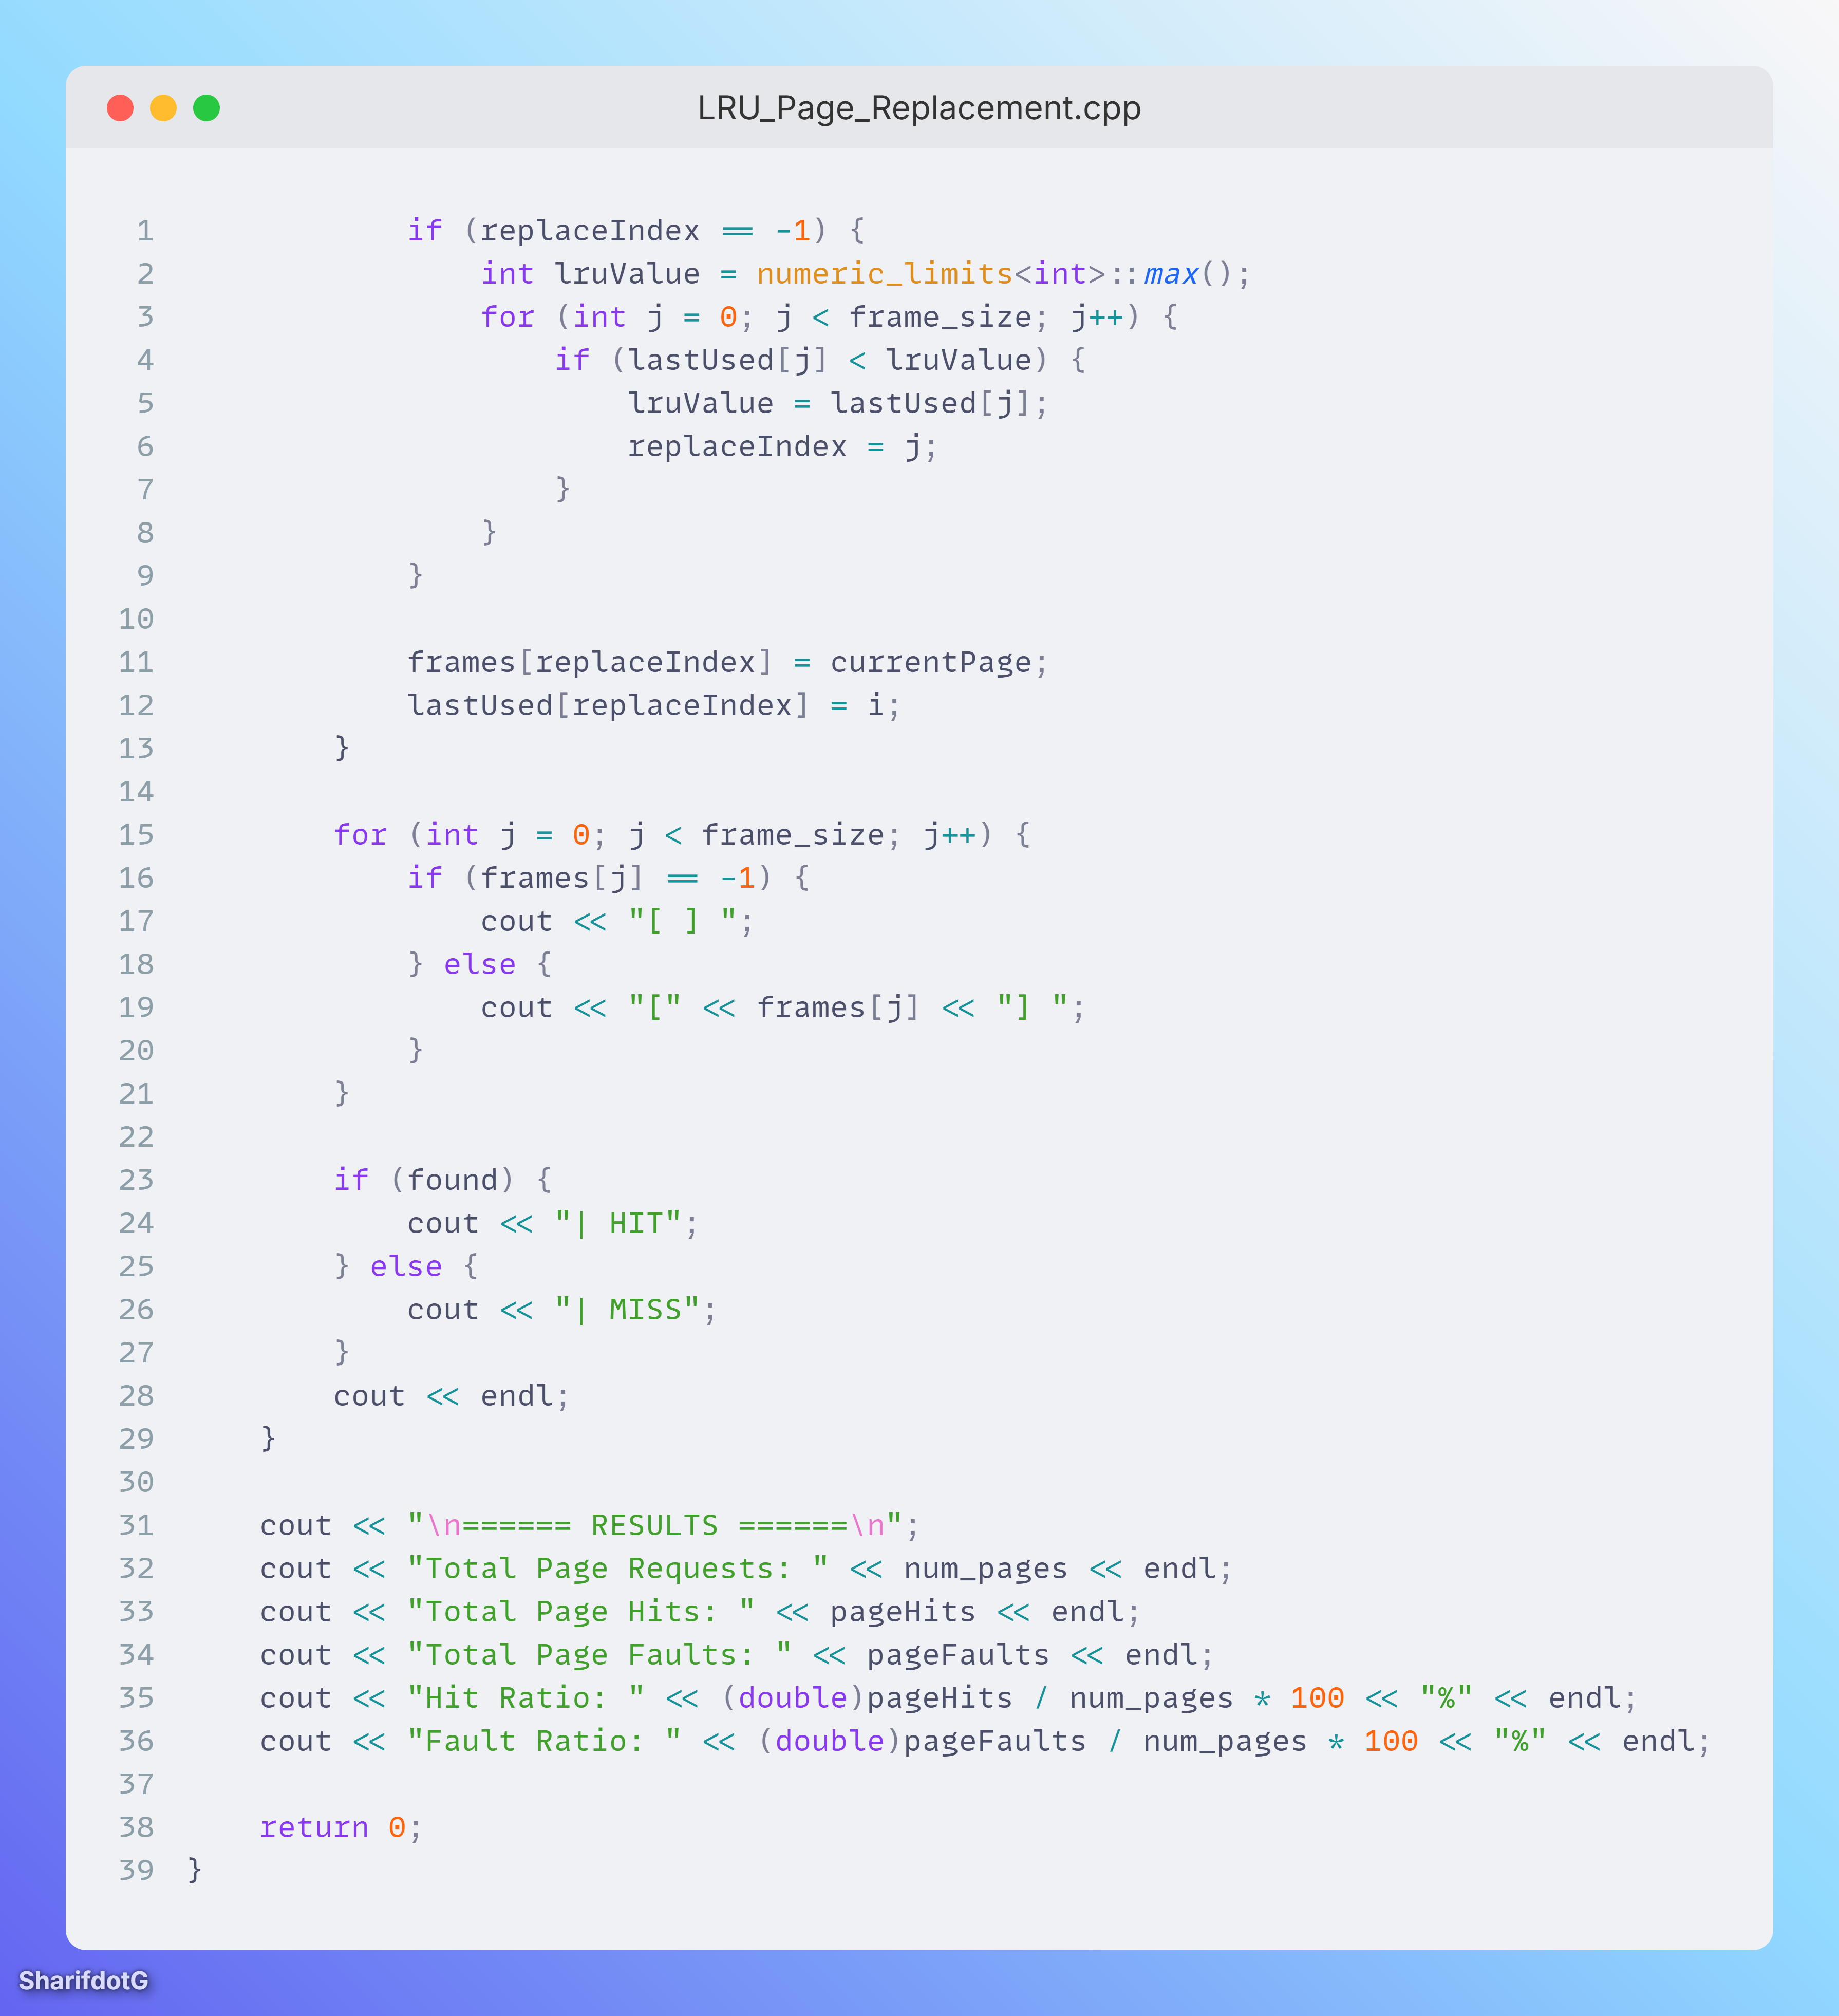
\includegraphics[width=0.85\textwidth]{Code2.png}
	\caption{LRU Page Replacement Source Code (Part 2)}
\end{figure}

\section{Output Screenshot}
\begin{figure}[H]
	\centering
	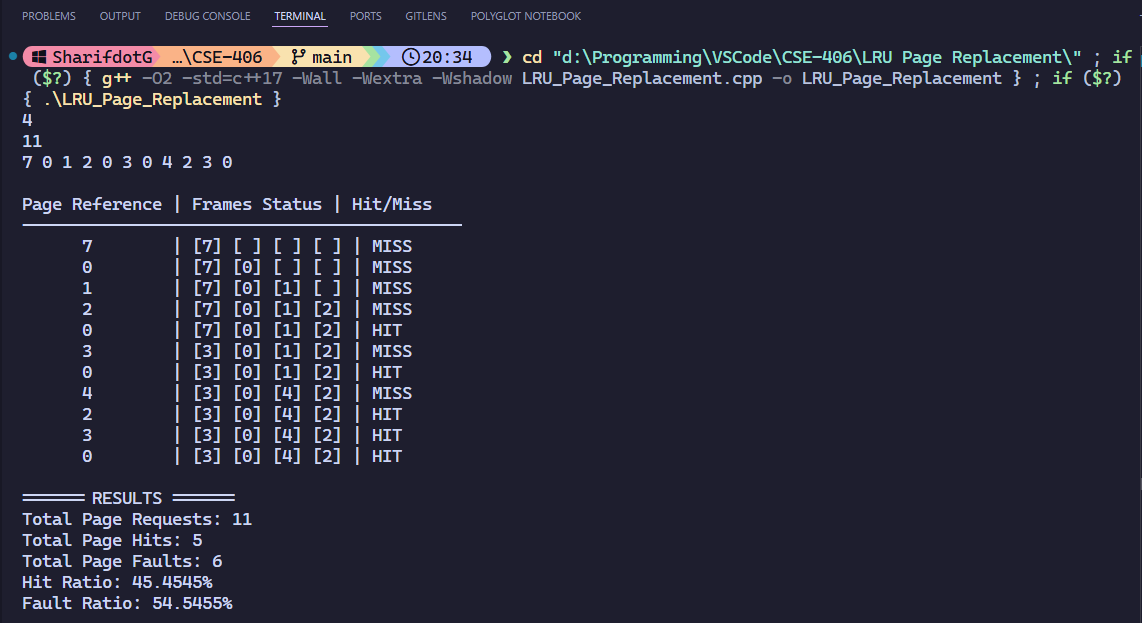
\includegraphics[width=0.9\textwidth]{Screenshot 2025-10-09 203619.png}
	\caption{LRU Program Output}
\end{figure}

\section{Discussion}
Working with the LRU policy highlighted how valuable temporal locality is for page replacement. Some of the key insights I recorded during the experiment are:

\begin{itemize}
		\item \textbf{Recency Tracking:} Maintaining the access timestamp for every frame guarantees that the algorithm always evicts the page that has stayed idle the longest, which aligns well with real workloads that reuse recently referenced pages.
		\item \textbf{Improved Hit Ratio:} Compared to FIFO, LRU preserved frequently accessed pages like 0 and 3, leading to five hits out of eleven references even with just four frames.
		\item \textbf{Overhead Considerations:} The implementation needs additional bookkeeping (the \texttt{lastUsed} array) to keep recency information up to date, adding a small computational overhead per access.
		\item \textbf{Deterministic Behaviour:} Given a fixed reference string, LRU produces a deterministic trace, making it easy to validate the simulator against manual calculations.
		\item \textbf{Comparison with MRU:} In scenarios where scans sweep through large data sets, MRU can outperform LRU, but for this string LRU clearly avoids wasting frames on rarely reused pages.
\end{itemize}

\section{Conclusion}
This lab solidified my understanding of the LRU page replacement approach and illustrated how intelligent eviction decisions can substantially reduce page faults. By tracking access recency, the simulator managed to retain hot pages and limit total faults to six for the given workload. Although LRU incurs bookkeeping overhead, the resulting hit ratio and predictable behaviour make it a strong baseline policy for demand paging systems. The experience also prepared me to evaluate more advanced approximations of LRU in future experiments.

\end{document}
